\chapter{Linear systems and Gaussian elimination}\label{ch:elimination}

Nearly every computation in this book — least squares, eigenvalue computations, and the neural-network training of part~IV — ends with a system of linear equations. This chapter builds the one algorithm that solves them honestly: Gaussian elimination. After it you will be able to (a) read a linear system two ways, as intersecting hyperplanes and as a combination of columns; (b) reduce any system to echelon form and read off whether it has zero, one, or infinitely many solutions; (c) package the work of elimination as the factorization $PA=LU$; and (d) say why elimination costs about $n^3$ operations and why a naive computer must swap rows to stay accurate.

\section{Two ways to see \texorpdfstring{$A\mathbf{x}=\mathbf{b}$}{Ax = b}}\label{sec:rowcol}

A \emph{linear system}\index{linear system} is a set of equations
\[
  a_{11}x_1 + a_{12}x_2 + \cdots + a_{1n}x_n = b_1,
  \quad\ldots\quad
  a_{m1}x_1 + a_{m2}x_2 + \cdots + a_{mn}x_n = b_m,
\]
which we compress into $A\mathbf{x}=\mathbf{b}$: the \emph{coefficient matrix}\index{coefficient matrix} $A$ is $m\times n$, $\mathbf{x}$ is the unknown column vector in $\mathbb{R}^n$, and $\mathbf{b}\in\mathbb{R}^m$ is given. Take the smallest non-trivial case, $m=n=2$:
\[
  2x - y = 0, \qquad -x + 2y = 3.
\]
There are two honest ways to look at it, and you need both.

\begin{description}
  \item[Row picture.] Each equation is a line\index{row picture} in the plane; solving means finding where the lines meet. Here they meet at the single point $(x,y)=(1,2)$.
  \item[Column picture.] Write the system as
  \(
    x\,\mathbf{a}_1 + y\,\mathbf{a}_2 = \mathbf{b}
  \),
  where $\mathbf{a}_1=(2,-1)$ and $\mathbf{a}_2=(-1,2)$ are the \emph{columns} of $A$\index{column picture}. Solving means finding the right weights: how many copies of each column add up to $\mathbf{b}=(0,3)$. The answer $x=1,\ y=2$ says $\mathbf{a}_1 + 2\mathbf{a}_2 = \mathbf{b}$.
\end{description}

\begin{figure}[htbp]
\centering
% Figure 1.1: row picture vs column picture of 2x - y = 0, -x + 2y = 3.
\begin{tikzpicture}[scale=1.0,>=stealth]
  % ---- row picture: two lines meet at (1,2) ----
  \begin{scope}[xshift=0cm,scale=0.85]
    \draw[->,gray] (-0.6,0) -- (3.0,0) node[below left] {\small $x$};
    \draw[->,gray] (0,-0.9) -- (0,3.4) node[below left] {\small $y$};
    \draw[thick] (-0.25,-0.5) -- (1.6,3.2) node[sloped,pos=0.86,above] {\small $2x-y=0$};
    \draw[thick,dashed] (-0.4,1.3) -- (3.0,3.0) node[sloped,pos=0.9,above] {\small $-x+2y=3$};
    \filldraw[accent] (1,2) circle (1.6pt) node[below right=-1pt] {\small $(1,2)$};
    \node at (1.2,-1.35) {\small (a) row picture: intersect};
  \end{scope}
  % ---- column picture: 1*a1 + 2*a2 = b ----
  \begin{scope}[xshift=6.4cm,scale=0.85]
    \draw[->,gray] (-1.8,0) -- (2.8,0) node[below left] {\small $x$};
    \draw[->,gray] (0,-1.8) -- (0,3.6) node[below left] {\small $y$};
    \draw[->,thick] (0,0) -- (2,-1) node[midway,below] {\small $\mathbf a_1$};
    \draw[->,thick,dashed] (0,0) -- (-1,2) node[midway,left] {\small $\mathbf a_2$};
    \draw[->,dotted,gray] (2,-1) -- (1,1);
    \draw[->,dotted,gray] (1,1) -- (0,3) node[midway,right] {\small $+2\mathbf a_2$};
    \draw[->,very thick,accent] (0,0) -- (0,3) node[midway,left] {\small $\mathbf b$};
    \node at (0.5,-2.15) {\small (b) column picture: $\mathbf a_1+2\mathbf a_2=\mathbf b$};
  \end{scope}
\end{tikzpicture}

\caption{Two pictures of the same $2\times2$ system. Notice that the \emph{weights} in the column picture (b) are exactly the coordinates of the meeting point in the row picture (a). The row picture shows what a solution \emph{is}; the column picture shows why one \emph{exists} — it exists precisely when $\mathbf{b}$ can be built from the columns.}
\label{fig:rowcol}
\end{figure}

The column picture is the one that scales. Three equations in three unknowns ask: is $\mathbf{b}$ a combination of three vectors in $\mathbb{R}^3$? If those columns fill out all of $\mathbb{R}^3$, every $\mathbf{b}$ is reachable and the system always has a solution. If the three columns happen to lie in one plane, only $\mathbf{b}$'s in that plane work — most systems are then unsolvable. The vector-spaces chapter turns this into the four fundamental subspaces; for now keep the image: \emph{$A\mathbf{x}$ is a combination of the columns of $A$ with weights $\mathbf{x}$}.

\begin{remark}
The row picture and column picture are the same arithmetic seen from two sides. Experienced readers switch between them without noticing. Practise the switch now, on paper, until it is automatic.
\end{remark}

\section{Elimination to echelon form}\label{sec:elim}

The row picture tells us what we want; elimination is how we get it. The idea is mechanical: use one equation to remove a variable from the equations below it, then repeat. Three moves — the \emph{elementary row operations}\index{row operation} — are legal because each leaves the solution set unchanged:
\begin{enumerate}
  \item add a multiple of one equation to another;
  \item multiply an equation by a non-zero number;
  \item swap two equations.
\end{enumerate}
Writing only the coefficients, in the \emph{augmented matrix}\index{augmented matrix} $[\,A\mid\mathbf{b}\,]$, we eliminate column by column until the system is \emph{upper triangular}\index{upper triangular} — in \emph{echelon form}\index{echelon form} — and then solve by \emph{back substitution}\index{back substitution}, bottom row upward.

\begin{example}\label{ex:threesys}
Solve the system
\[
  x + 2y + z = 7,\qquad
  3x + 8y + z = 17,\qquad
  2y + 3z = 11.
\]
\textbf{Strategy.} Use the $1$ in position $(1,1)$ — the first \emph{pivot} — to clear column~1: subtract $3\times$~row~1 from row~2. Row~3 already has a zero in column~1, so it is left alone — a step may be a no-op. Then subtract row~2 from row~3 to clear column~2. Finally read $z$, then $y$, then $x$ from the bottom up.
\begin{solution}
The augmented matrix and its two elimination steps appear in figure~\ref{fig:elimsteps}:
\[
  \left[\begin{array}{ccc|c} 1 & 2 & 1 & 7\\ 3 & 8 & 1 & 17\\ 0 & 2 & 3 & 11\end{array}\right]
  \xrightarrow{R_2-3R_1}
  \left[\begin{array}{ccc|c} 1 & 2 & 1 & 7\\ 0 & 2 & -2 & -4\\ 0 & 2 & 3 & 11\end{array}\right]
  \xrightarrow{R_3-R_2}
  \left[\begin{array}{ccc|c} 1 & 2 & 1 & 7\\ 0 & 2 & -2 & -4\\ 0 & 0 & 5 & 15\end{array}\right].
\]
Back substitution: $5z=15$ gives $z=3$; then $2y - 2(3) = -4$ gives $y=1$; then $x + 2(1) + 3 = 7$ gives $x=2$. The solution is $(x,y,z)=(2,1,3)$. Check: $2+2+3=7$; $6+8+3=17$; $2+9=11$. \checkmark
\end{solution}
\end{example}

\begin{figure}[htbp]
\centering
% Figure 1.2: elimination on the worked-example matrix, three states.
\begin{tikzpicture}[every node/.style={inner sep=1pt}]
\node (s0) {\footnotesize$\left[\begin{array}{ccc|c}
  \cellcolor{accentsoft}1 & 2 & 1 & 7\\
  3 & 8 & 1 & 17\\
  0 & 2 & 3 & 11\end{array}\right]$};
\node[below=2pt of s0] {\small start};
\node[right=2.6em of s0] (s1) {\footnotesize$\left[\begin{array}{ccc|c}
  1 & 2 & 1 & 7\\
  0 & \cellcolor{accentsoft}2 & -2 & -4\\
  0 & 2 & 3 & 11\end{array}\right]$};
\node[below=2pt of s1] {\small after column 1};
\node[right=2.6em of s1] (s2) {\footnotesize$\left[\begin{array}{ccc|c}
  1 & 2 & 1 & 7\\
  0 & 2 & -2 & -4\\
  0 & 0 & \cellcolor{accentsoft}5 & 15\end{array}\right]$};
\node[below=2pt of s2] {\small echelon form};
\draw[->,thick] (s0) -- (s1) node[midway,above,align=center]
  {\scriptsize $R_2\!-\!3R_1$\\[-2pt]\scriptsize ($R_3$ already $0$)};
\draw[->,thick] (s1) -- (s2) node[midway,above] {\scriptsize $R_3\!-\!R_2$};
\end{tikzpicture}

\caption{Elimination on example~\ref{ex:threesys}, one state per step. Notice the shaded \emph{pivots} marching down the diagonal, and that only the entries below the current pivot are touched. The third state is upper triangular: back substitution can start.}
\label{fig:elimsteps}
\end{figure}

Two bookkeeping rules make this reliable on paper. First, \emph{one column at a time, left to right} — never clear a column above the current pivot. Second, \emph{record each multiplier}\index{multiplier}: the number $\ell_{ik}$ that makes $R_i \gets R_i - \ell_{ik}R_k$ cancel the $(i,k)$ entry is $\ell_{ik}=a_{ik}/a_{kk}$. Those multipliers are not scratch work; section~\ref{sec:lu} shows they \emph{are} the matrix $L$.

\begin{lstlisting}[language=Python,caption={Forward elimination in plain Python on example~\ref{ex:threesys}, checked against \texttt{numpy}. File: \texttt{code/ch01\_forward\_elimination.py}.},label={lst:fwdelim}]
import numpy as np

A = np.array([[1., 2., 1.],
              [3., 8., 1.],
              [0., 2., 3.]])
b = np.array([7., 17., 11.])
n = len(b)

Ab = np.column_stack([A, b])     # the augmented matrix [A | b]
for col in range(n - 1):         # eliminate below each pivot, left to right
    for row in range(col + 1, n):
        m = Ab[row, col] / Ab[col, col]   # this multiplier kills Ab[row, col]
        Ab[row] -= m * Ab[col]
print("echelon form [U | c]:")
print(Ab)

x = np.zeros(n)                  # back substitution reads U bottom to top
for row in range(n - 1, -1, -1):
    x[row] = (Ab[row, n] - Ab[row, row + 1:n] @ x[row + 1:n]) / Ab[row, row]
print("x =", x)
print("np.linalg.solve agrees:", np.linalg.solve(A, b))
print("residual ||Ax-b|| =", np.linalg.norm(A @ x - b))
\end{lstlisting}

\begin{lstlisting}[caption={Output of listing~\ref{lst:fwdelim}. The echelon form matches figure~\ref{fig:elimsteps} exactly; pivots $1,2,5$.}]
echelon form [U | c]:
[[ 1.  2.  1.  7.]
 [ 0.  2. -2. -4.]
 [ 0.  0.  5. 15.]]
x = [2. 1. 3.]
np.linalg.solve agrees: [2. 1. 3.]
residual ||Ax-b|| = 0.0
\end{lstlisting}

\begin{exercise}[easy]
By hand, eliminate
\[
  x + 2y + z = 6,\qquad
  2x + y + 2z = 6,\qquad
  x - y + z = 2,
\]
to echelon form, then back-substitute. Write down the three pivots and every multiplier you used.
\end{exercise}

\section{Pivots, free variables, and the shape of a solution set}\label{sec:shape}

In example~\ref{ex:threesys} every column had a pivot. That need not happen — and what happens instead is the whole story of a linear system.

\begin{definition}\label{def:pivot}
A \emph{pivot}\index{pivot} is the first non-zero entry in its row once the matrix is in echelon form. The columns containing pivots are \emph{pivot columns}; the remaining variables are \emph{free variables}\index{free variable} — they may take any value, and the pivot variables are then determined by back substitution. The number of pivots is the \emph{rank}\index{rank} of $A$.
\end{definition}

Reading the echelon form $[\,U\mid\mathbf{c}\,]$ settles existence and uniqueness at a glance:
\begin{itemize}
  \item a row $[\,0\ \cdots\ 0 \mid c\,]$ with $c\neq0$ says $0=c$: \textbf{no solution};
  \item otherwise, if every variable column is a pivot column: \textbf{exactly one solution};
  \item otherwise, free variables exist: \textbf{infinitely many solutions}, and each free variable adds one degree of freedom to the solution set.
\end{itemize}

\begin{figure}[htbp]
\centering
% Figure 1.3: the four shapes a solution set can take.
\begin{tikzpicture}[scale=0.78,>=stealth,
  ax/.style={->,gray}]
  % (a) unique solution: a point
  \begin{scope}
    \draw[ax] (0,0) -- (1.7,0);\draw[ax] (0,0) -- (0,1.5);\draw[ax] (0,0) -- (-0.9,-0.7);
    \filldraw[accent] (0.55,0.6) circle (2.2pt);
    \node at (0.4,-1.35) {\small (a) point};
  \end{scope}
  % (b) one free variable: a line
  \begin{scope}[xshift=3.6cm]
    \draw[ax] (0,0) -- (1.7,0);\draw[ax] (0,0) -- (0,1.5);\draw[ax] (0,0) -- (-0.9,-0.7);
    \draw[thick] (-0.6,-0.1) -- (1.5,1.2);
    \node at (0.45,-1.35) {\small (b) line};
  \end{scope}
  % (c) two free variables: a plane
  \begin{scope}[xshift=7.4cm]
    \draw[ax] (0,0) -- (1.7,0);\draw[ax] (0,0) -- (0,1.5);\draw[ax] (0,0) -- (-0.9,-0.7);
    \draw[thick,fill=accentsoft] (-0.6,0.15) -- (0.7,0.65) -- (1.6,1.25) -- (0.3,0.75) -- cycle;
    \node at (0.5,-1.35) {\small (c) plane};
  \end{scope}
  % (d) inconsistent: parallel planes, empty set
  \begin{scope}[xshift=11.2cm]
    \draw[thick,fill=accentsoft] (-0.6,0.1) -- (0.7,0.6) -- (1.6,1.2) -- (0.3,0.7) -- cycle;
    \draw[thick,fill=graybg] (-0.5,-0.6) -- (0.8,-0.1) -- (1.7,0.5) -- (0.4,0.0) -- cycle;
    \node at (0.55,-1.35) {\small (d) empty set};
  \end{scope}
\end{tikzpicture}

\caption{The four shapes a solution set can take, drawn in $\mathbb{R}^3$. Notice there is no ``two solutions'' case: the moment two distinct points solve the system, the whole line through them does. A solution set is always empty, a point, a line, a plane, \dots — never a finite blob.}
\label{fig:solgeom}
\end{figure}

\begin{example}\label{ex:singular}
Find all solutions of $A\mathbf{x}=\mathbf{b}$ for
\[
  A=\begin{bmatrix} 1 & 2 & 1\\ 2 & 4 & 2\\ 1 & 1 & 0\end{bmatrix},
  \qquad \mathbf{b}=\begin{bmatrix} 4\\ 8\\ 1\end{bmatrix}.
\]
\textbf{Strategy.} Eliminate as usual and watch for a row of zeros: it signals a redundant (or contradictory) equation. Then separate pivot and free variables per definition~\ref{def:pivot} and parametrize.
\begin{solution}
$R_2-2R_1$ produces the zero row $[\,0\ 0\ 0\mid0\,]$ — consistent, since $0=0$. Then $R_3-R_1=[\,0\ -1\ -1\mid-3\,]$, and the echelon form is
\[
  \left[\begin{array}{ccc|c} 1 & 2 & 1 & 4\\ 0 & -1 & -1 & -3\\ 0 & 0 & 0 & 0\end{array}\right].
\]
Pivots sit in columns 1 and 2, so $x_3=t$ is free. Back substitution: $x_2=3-t$ and $x_1=4-2x_2-x_3=-2+t$. All solutions:
\[
  \mathbf{x} = \begin{bmatrix} -2\\ 3\\ 0\end{bmatrix} + t\begin{bmatrix} 1\\ -1\\ 1\end{bmatrix},
  \qquad t\in\mathbb{R},
\]
a line in $\mathbb{R}^3$ — case (b) of figure~\ref{fig:solgeom}. The vector $\mathbf{x}_p=(-2,3,0)$ is a \emph{particular solution}\index{particular solution}; the vector $(1,-1,1)$ spans the \emph{null space}\index{null space} of $A$ (check: $A(1,-1,1)^{T}=\mathbf{0}$).
\end{solution}
\end{example}

That decomposition in the last line of example~\ref{ex:singular} is not a coincidence — it is the structural theorem of the chapter.

\begin{theorem}\label{thm:affinesol}
If $\mathbf{x}_p$ is one solution of $A\mathbf{x}=\mathbf{b}$, then the complete solution set is
\[
  \{\,\mathbf{x}_p + \mathbf{x}_h : \mathbf{x}_h \in N(A)\,\},
\]
where $N(A)=\{\mathbf{x}:A\mathbf{x}=\mathbf{0}\}$ is the null space of $A$.
\end{theorem}

\begin{proof}
Take any $\mathbf{x}_h\in N(A)$: then $A(\mathbf{x}_p+\mathbf{x}_h)=A\mathbf{x}_p+A\mathbf{x}_h=\mathbf{b}+\mathbf{0}=\mathbf{b}$, so every such vector is a solution. Conversely, if $\mathbf{x}$ solves the system, write $\mathbf{x}=\mathbf{x}_p+(\mathbf{x}-\mathbf{x}_p)$ and note $A(\mathbf{x}-\mathbf{x}_p)=\mathbf{b}-\mathbf{b}=\mathbf{0}$, so $\mathbf{x}-\mathbf{x}_p\in N(A)$.
\end{proof}

This is why figure~\ref{fig:solgeom} shows only flats: the solution set is the null space — always a flat through the origin — shifted to pass through $\mathbf{x}_p$.

\begin{exercise}[medium]
For the same matrix $A$ as example~\ref{ex:singular}, try $\mathbf{b}=(4,9,1)^{T}$. What row appears in elimination, and what does it say about the solution set? Then pick any $\mathbf{b}$ in the plane $2b_1-b_2=0$ and confirm the system is solvable.
\end{exercise}

\begin{example}\label{ex:balance}
Balance the reaction $\mathrm{Fe}_2\mathrm{O}_3 + \mathrm{CO} \to \mathrm{Fe} + \mathrm{CO}_2$:
find whole numbers $a,b,c,d$ with
$a\,\mathrm{Fe}_2\mathrm{O}_3 + b\,\mathrm{CO} \to c\,\mathrm{Fe} + d\,\mathrm{CO}_2$.
\par\smallskip
\textbf{Strategy.} Each element gives one linear equation in the four
coefficients. Four unknowns, three equations, zero right-hand sides ---
this is the homogeneous case of section~\ref{sec:shape}, so the answer
will be a free-variable family, not a single vector.
\begin{solution}
Fe: $2a=c$; C: $b=d$; O: $3a+b=2d$. The C and Fe equations hand $b=d$
and $c=2a$; the O equation becomes $3a+d=2d$, i.e.\ $d=3a$, so
$b=3a$ too. Every solution is $(a,b,c,d)=a\,(1,3,2,3)$ --- the solution
set is a \emph{ray}, exactly the null space of the $3\times4$ atom
matrix (figure~\ref{fig:balance}). There is no ``the'' answer until the
physical rule arrives: chemists want the smallest whole numbers, so
$a=1$ and
\[
  \mathrm{Fe}_2\mathrm{O}_3 + 3\,\mathrm{CO} \longrightarrow 2\,\mathrm{Fe} + 3\,\mathrm{CO}_2.
\]
Check the atoms: Fe $2=2$, C $3=3$, O $3+3=6$. \checkmark
\end{solution}
\end{example}

\begin{figure}[ht]\centering
% Figure 1.5: chemical balancing is a homogeneous system.
% The solution set is a ray through the origin; whole-number answers
% are the lattice points on it. The smallest one is the balance.
\begin{tikzpicture}[scale=0.9,>=stealth]
  % left panel: the atom bookkeeping
  \begin{scope}
    \node[anchor=west,font=\small] at (0,3.1) {$a\,\mathrm{Fe}_2\mathrm{O}_3 + b\,\mathrm{CO} \longrightarrow c\,\mathrm{Fe} + d\,\mathrm{CO}_2$};
    \node[anchor=west,font=\small] at (0.2,2.4) {Fe: $2a = c$};
    \node[anchor=west,font=\small] at (0.2,1.8) {C:  $b = d$};
    \node[anchor=west,font=\small] at (0.2,1.2) {O:  $3a + b = 2d$};
    \node[anchor=west,font=\small] at (0.2,0.4) {one free variable $a$:\ \ $b=d=3a,\ c=2a$};
    \node at (2.1,-0.6) {\small atoms $\to$ equations};
  \end{scope}
  % right panel: the solution ray in the (a,b) projection
  \begin{scope}[xshift=7.6cm]
    \draw[->,gray] (0,0) -- (3.2,0) node[right,font=\small] {$a$};
    \draw[->,gray] (0,0) -- (0,3.2) node[above,font=\small] {$b$};
    \draw[thick] (0,0) -- (3.0,3.0) node[pos=0.9,above left=-2pt,font=\small] {$b=3a$};
    \filldraw[accent] (1,1) circle (2.4pt) node[right=2pt,font=\small] {$a{=}1$: $(1,3,2,3)$};
    \filldraw[gray] (2,2) circle (1.8pt) node[right=2pt,font=\small] {$a{=}2$};
    \filldraw[gray] (3,3) circle (1.8pt) node[right=2pt,font=\small] {$a{=}3$};
    \node at (1.7,-0.8) {\small the ray $t\,(1,3,2,3)$};
    \node at (1.7,-1.35) {\small integer points = valid balances};
  \end{scope}
\end{tikzpicture}

\caption{Chemical balancing is elimination on a homogeneous system.
Notice the pattern of figure~\ref{fig:solgeom}(b) reappearing: one free
variable means a ray of answers, and the ``smallest whole-number'' rule
picks the first lattice point on it.}
\label{fig:balance}
\end{figure}

\section{LU factorization (and \texorpdfstring{$PA=LU$}{PA = LU} with row exchanges)}\label{sec:lu}

Here is the observation that turns elimination from a procedure into a theory. Each step ``subtract $\ell_{ik}$ times row $k$ from row $i$'' can itself be undone by a matrix. Suppose elimination needs no row swaps. Then the multipliers $\ell_{ik}$, placed in a lower-triangular matrix $L$\index{L matrix} with 1s on the diagonal, satisfy
\[
  A = LU, \qquad\text{$L$ lower triangular, $U$ upper triangular.}
\]
This is the \emph{LU factorization}\index{LU factorization}: $U$ is exactly the echelon form elimination produced, and $L$ is nothing but the multiplier record kept below the diagonal. Solving $A\mathbf{x}=\mathbf{b}$ becomes two triangular solves — forward substitution $L\mathbf{c}=\mathbf{b}$, then back substitution $U\mathbf{x}=\mathbf{c}$ — and the factorization is reusable: a new $\mathbf{b}$ costs only $O(n^2)$, not another elimination.

If a pivot position is zero while nonzero entries sit below it, swap rows first. Collecting all swaps into a \emph{permutation matrix}\index{permutation matrix} $P$ gives the complete statement: \emph{every} square matrix admits
\[
  PA = LU.
\]

\begin{example}\label{ex:lu}
Factor
\(
  A=\begin{bmatrix} 1 & 1 & 2\\ 2 & 2 & 3\\ 1 & 0 & 1\end{bmatrix}
\)
as $PA=LU$.
\textbf{Strategy.} Column 1 is fine (pivot 1, eliminate with multipliers 2 and 1). Column 2 then has a $0$ in the pivot position — so swap rows 2 and 3 \emph{before} eliminating, and keep the swap in $P$.
\begin{solution}
After $R_2-2R_1$ and $R_3-R_1$:
\[
  \begin{bmatrix} 1 & 1 & 2\\ 0 & 0 & -1\\ 0 & -1 & -1\end{bmatrix}
  \xrightarrow{\text{swap }R_2\leftrightarrow R_3}
  \begin{bmatrix} 1 & 1 & 2\\ 0 & -1 & -1\\ 0 & 0 & -1\end{bmatrix}=U.
\]
It is cleaner to apply the swap to $A$ up front — eliminate $PA$ where $P$ exchanges rows 2 and 3:
\[
  PA=\begin{bmatrix} 1 & 1 & 2\\ 1 & 0 & 1\\ 2 & 2 & 3\end{bmatrix},\quad
  L=\begin{bmatrix} 1 & 0 & 0\\ 1 & 1 & 0\\ 2 & 0 & 1\end{bmatrix},\quad
  U=\begin{bmatrix} 1 & 1 & 2\\ 0 & -1 & -1\\ 0 & 0 & -1\end{bmatrix}.
\]
Multipliers went straight into $L$ (below-diagonal, in the order the rows ended up). Check $LU=PA$: row 2 of $LU$ is $1\cdot(1,1,2)+1\cdot(0,-1,-1)=(1,0,1)$ — the second row of $PA$. \checkmark
\end{solution}
\end{example}

\begin{lstlisting}[language=Python,caption={Verifying example~\ref{ex:lu} and comparing with \texttt{scipy.linalg.lu}. File: \texttt{code/ch01\_lu\_factorization.py}.},label={lst:lu}]
import numpy as np
from scipy.linalg import lu

A = np.array([[1., 1., 2.], [2., 2., 3.], [1., 0., 1.]])
P = np.array([[1., 0., 0.], [0., 0., 1.], [0., 1., 0.]])  # swaps rows 2,3
L = np.array([[1., 0., 0.], [1., 1., 0.], [2., 0., 1.]])
U = np.array([[1., 1., 2.], [0., -1., -1.], [0., 0., -1.]])

print("PA =\n", P @ A)
print("L @ U =\n", L @ U)
print("||PA - LU|| =", np.linalg.norm(P @ A - L @ U))

P_sp, L_sp, U_sp = lu(A)   # scipy picks its own pivots
print("scipy P =\n", P_sp)
print("||P_sp A - L_sp U_sp|| =", np.linalg.norm(P_sp @ A - L_sp @ U_sp))
\end{lstlisting}

\begin{lstlisting}[caption={Output of listing~\ref{lst:lu}. Our hand factorization is exact; scipy chooses different pivots — a different, equally valid $PA=LU$.}]
PA =
 [[1. 1. 2.]
 [1. 0. 1.]
 [2. 2. 3.]]
L @ U =
 [[1. 1. 2.]
 [1. 0. 1.]
 [2. 2. 3.]]
||PA - LU|| = 0.0
scipy P =
 [[0. 0. 1.]
 [1. 0. 0.]
 [0. 1. 0.]]
||P_sp A - L_sp U_sp|| = 0.0
\end{lstlisting}

\begin{remark}
The scipy output makes an important point: $PA=LU$ is not unique. Any order you pull the rows down in gives a valid factorization; \texttt{scipy} picks pivots by the rule of section~\ref{sec:cost}, not by the order we happened to choose.
\end{remark}

\begin{exercise}[medium]
Factor $A=\begin{bmatrix} 2 & 1 & 0\\ 4 & 3 & 1\\ 0 & 2 & 1\end{bmatrix}$ as $A=LU$ (no swaps needed). Then solve $A\mathbf{x}=(4,10,3)^{T}$ by solving $L\mathbf{c}=\mathbf{b}$ then $U\mathbf{x}=\mathbf{c}$.
\end{exercise}

\begin{example}\label{ex:twob}
You factored
\(
  A=\begin{bmatrix} 2 & 1 & 0\\ 4 & 3 & 1\\ 0 & 2 & 1\end{bmatrix}
  =\underbrace{\begin{bmatrix} 1 & 0 & 0\\ 2 & 1 & 0\\ 0 & 2 & 1\end{bmatrix}}_L
   \underbrace{\begin{bmatrix} 2 & 1 & 0\\ 0 & 1 & 1\\ 0 & 0 & -1\end{bmatrix}}_U
\)
once. Now two queries arrive: solve $A\mathbf{x}=\mathbf{b}_1$ for
$\mathbf{b}_1=(4,10,3)^{T}$ and $A\mathbf{x}=\mathbf{b}_2$ for
$\mathbf{b}_2=(1,3,2)^{T}$. What does the second one cost?
\par\smallskip
\textbf{Strategy.} Do not re-eliminate. Each solve is two triangular
systems: $L\mathbf{c}=\mathbf{b}$ forward, $U\mathbf{x}=\mathbf{c}$
back (figure~\ref{fig:twob}).
\begin{solution}
$\mathbf{b}_1$: $c_1=4$, $c_2=10-2\cdot4=2$, $c_3=3-2\cdot2=-1$; then
$-x_3=-1\Rightarrow x_3=1$, $x_2=2-1=1$, $2x_1=4-1\Rightarrow x_1=\tfrac32$.
So $\mathbf{x}_1=(\tfrac32,1,1)^{T}$.
$\mathbf{b}_2$: $c_1=1$, $c_2=3-2=1$, $c_3=2-2=0$; then $x_3=0$,
$x_2=1$, $2x_1=1-1\Rightarrow x_1=0$. So $\mathbf{x}_2=(0,1,0)^{T}$ ---
and indeed $A(0,1,0)^{T}=(1,3,2)^{T}$. \checkmark
The second solve cost two $O(n^2)$ sweeps --- nothing like the
$\tfrac23 n^3$ of elimination. This is why libraries return a
factorization object, not an answer.
\end{solution}
\end{example}

\begin{figure}[ht]\centering
% Figure 1.6: factor once, solve per right-hand side.
% The expensive stage (elimination, O(n^3)) runs once; each new b
% rides two O(n^2) triangular solves.
\begin{tikzpicture}[scale=1.0,>=stealth,
  box/.style={draw,thick,rounded corners=2pt,inner sep=5pt,align=center,font=\small},
  cost/.style={font=\footnotesize,gray}]
  \node[box] (a) at (0,0) {$A$ and all $\mathbf{b}$'s up front};
  \node[box,fill=accentsoft] (lu) at (4.6,0) {$PA=LU$ \\ factor once};
  \node[cost] at (4.6,-0.95) {$\tfrac23 n^3$ flops};
  \node[box] (fwd1) at (8.9,1.1) {$L\mathbf{c}_1=\mathbf{b}_1$};
  \node[box] (bwd1) at (8.9,0.0) {$U\mathbf{x}_1=\mathbf{c}_1$};
  \node[box] (fwd2) at (8.9,-1.6) {$L\mathbf{c}_2=\mathbf{b}_2$};
  \node[box] (bwd2) at (8.9,-2.7) {$U\mathbf{x}_2=\mathbf{c}_2$};
  \draw[->,thick] (a) -- (lu);
  \draw[->,thick] (lu.east) -- (fwd1.west);
  \draw[->,thick] (fwd1) -- (bwd1);
  \draw[->,thick] (lu.east) -- (fwd2.west);
  \draw[->,thick] (fwd2) -- (bwd2);
  \node[cost] at (8.9,0.55) {$2n^2$ flops};
  \node[cost] at (8.9,-2.15) {$2n^2$ flops};
  \node[font=\small,align=center] at (4.6,-3.4) {a third $\mathbf{b}$? two more triangular solves ---\\ no new factorization};
\end{tikzpicture}

\caption{Factor once, solve per right-hand side. Notice where the
$O(n^3)$ sits: entirely in the factorization. Every later $\mathbf{b}$
pays only triangular-solve prices.}
\label{fig:twob}
\end{figure}

\section{Cost and stability: why elimination is \texorpdfstring{$O(n^3)$}{O(n\string^3)} and why we pivot}\label{sec:cost}

\paragraph{The count.} To clear column $k$ of an $n\times n$ system you touch the lower-right $(n-k)\times(n-k)$ block: about $(n-k)^2$ multiply-add pairs. Summing over columns,
\[
  \sum_{k=1}^{n-1}(n-k)^2 = \frac{n(n-1)(2n-1)}{6} \approx \frac{n^3}{3}.
\]
So elimination costs about $n^3/3$ multiply-add steps — cubic\index{flop count}\index{computational complexity}. That scaling decides feasibility: doubling $n$ multiplies the work by eight, so $n=10^4$ is fine on a laptop while $n=10^6$ is not (structured matrices excepted — see the exercises).

\begin{lstlisting}[language=Python,caption={Timing our loop-based elimination against \texttt{np.linalg.solve}. File: \texttt{code/ch01\_cost\_scaling.py}.},label={lst:cost}]
import time
import numpy as np

def eliminate(A, b):
    n = len(b)
    Ab = np.column_stack([A, b])
    for col in range(n - 1):
        for row in range(col + 1, n):
            Ab[row] -= (Ab[row, col] / Ab[col, col]) * Ab[col]
    return Ab

np.linalg.solve(np.eye(3), np.ones(3))  # BLAS warm-up
print(f"{'n':>5} {'ours (s)':>10} {'solve (s)':>10}")
for n in [50, 100, 200, 400]:
    rng = np.random.default_rng(0)
    A, b = rng.standard_normal((n, n)), rng.standard_normal(n)
    t0 = time.perf_counter(); eliminate(A, b); t1 = time.perf_counter()
    t2 = time.perf_counter(); np.linalg.solve(A, b); t3 = time.perf_counter()
    print(f"{n:>5} {t1-t0:>10.4f} {t3-t2:>10.4f}")
\end{lstlisting}

\begin{lstlisting}[caption={Output of listing~\ref{lst:cost}. Each doubling of $n$ multiplies our time by roughly 4--5 in this range (the pure-Python per-operation overhead masks the asymptotic factor of 8; the fitted log-log slope is $\approx2.2$), while LAPACK behind \texttt{np.linalg.solve} is two orders of magnitude faster and its measured slope at larger $n$ is $\approx3.1$.}]
    n   ours (s)  solve (s)
   50     0.0008     0.0035
  100     0.0031     0.0002
  200     0.0141     0.0002
  400     0.0648     0.0007
\end{lstlisting}

\begin{figure}[htbp]
\centering
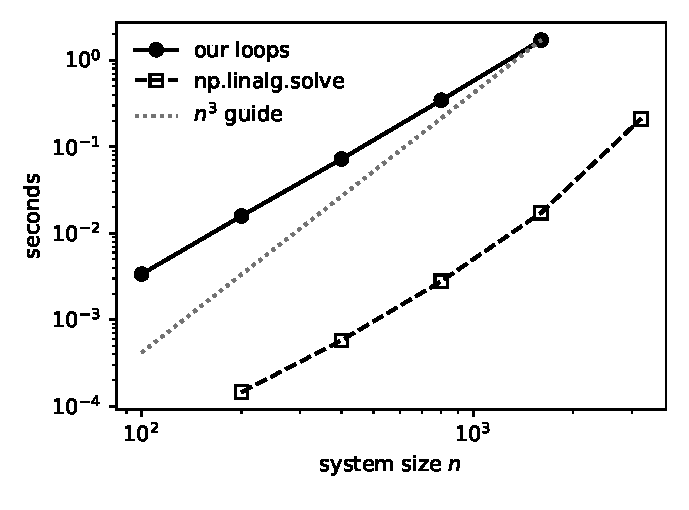
\includegraphics[width=0.75\linewidth]{figures/ch01_cost.pdf}
\caption{Measured cost of elimination vs $n$ on log-log axes, regenerated by \texttt{code/ch01\_cost\_figure.py}. Notice both curves trending toward the dotted $n^3$ guide: the algorithms differ only in their constant, not their shape. A slope of 3 on these axes is what ``cubic'' looks like.}
\label{fig:cost}
\end{figure}

\paragraph{The stability problem.} The count says nothing about whether the answer is \emph{right}. Floating-point arithmetic rounds every operation, and elimination can amplify rounding catastrophically when a pivot is tiny. Consider
\[
  \begin{bmatrix} 10^{-20} & 1\\ 1 & 1\end{bmatrix}\begin{bmatrix} x\\ y\end{bmatrix}=\begin{bmatrix} 1\\ 2\end{bmatrix},
  \qquad\text{true answer } x\approx1,\ y\approx1.
\]
Eliminating without a swap uses multiplier $10^{20}$: $R_2-10^{20}R_1$ gives $(1-10^{20})y=2-10^{20}$. In double precision $1-10^{20}=-10^{20}$, so $y=1$ exactly — and then the first equation reports $x=(1-y)/10^{-20}=0$. Plausible-looking output, confidently wrong. Swap the rows first and both multipliers stay below 1, giving $x\approx1$, $y\approx1$.

\begin{figure}[htbp]
\centering
% Figure 1.4: a tiny pivot without a swap produces a confidently wrong answer.
\begin{tikzpicture}[box/.style={draw,rounded corners=1pt,inner sep=4pt,align=center,font=\small},
  >=stealth]
\node[box,fill=amberbg] (p) {pivot $10^{-20}$\\[-2pt]\scriptsize tiny};
\node[box,fill=amberbg,right=1.1em of p] (m) {multiplier $10^{20}$\\[-2pt]\scriptsize huge};
\node[box,fill=amberbg,right=1.1em of m] (c) {$y\gets 1$\\[-2pt]\scriptsize plausible};
\node[box,fill=amberbg,right=1.1em of c] (w) {$x\gets(1-y)/10^{-20}=0$\\[-2pt]\scriptsize wrong: true $x\approx1$};
\draw[->,thick,amber] (p) -- (m);\draw[->,thick,amber] (m) -- (c);\draw[->,thick,amber] (c) -- (w);
\node[box,fill=goodbg,below=1.4em of m] (fix) {swap rows first: pivot $1$, multipliers $\le1$};
\draw[->,thick,good] (p.south) |- (fix.west);
\draw[->,thick,good] (fix.east) -| (w.south);
\end{tikzpicture}

\caption{How a tiny pivot destroys an answer, and the one-line fix. Notice the failure is silent — every intermediate number looks reasonable. This is why production solvers never take the diagonal entry as pivot blindly.}
\label{fig:pivfail}
\end{figure}

The fix is \emph{partial pivoting}\index{partial pivoting}: at each column, swap the largest-magnitude available entry into the pivot position. This keeps every multiplier $|\ell_{ik}|\le1$, which bounds how much rounding can grow (the \emph{growth factor}\index{growth factor} stays small for essentially all real problems). It costs a comparison per row — negligible against $n^3$ — and it is why \texttt{np.linalg.solve} computes $PA=LU$ with pivoting rather than the naive $LU$ of section~\ref{sec:lu}.

\begin{exercise}[hard]
Run the $10^{-20}$ system in Python three ways: no pivoting, with the row swap, and \texttt{np.linalg.solve}. Report the three $x$-values. Then replace $10^{-20}$ by $10^{-8}$: at what pivot size does the no-swap answer recover, and why?
\end{exercise}

\section{Hand derivation}\label{sec:handderiv}

Close the interpreter. Prove theorem~\ref{thm:affinesol} from scratch: the solution set of $A\mathbf{x}=\mathbf{b}$ is a particular solution plus the whole null space.
\begin{enumerate}
  \item Show that the set $S=\{\mathbf{x}_p+\mathbf{x}_h:\mathbf{x}_h\in N(A)\}$ contains only solutions (the $S\subseteq\{\text{solutions}\}$ direction).
  \item Show that every solution lies in $S$.
  \item Apply it: for example~\ref{ex:singular}, verify directly that the difference of any two solutions you can name is a multiple of $(1,-1,1)^{T}$.
  \item Conclude the count: if $A$ is $m\times n$ of rank $r$, the solution set (when non-empty) is a flat of dimension $n-r$. Why does that make ``exactly two solutions'' impossible?
\end{enumerate}

\section{Common mistakes}\label{sec:mistakes}

\begin{tripwire}[Sign errors in elimination bookkeeping]
Subtracting a multiple of a row the wrong way — $R_3+R_1$ when you meant $R_3-R_1$ — is the single most common error by hand. Defence: after each step, \emph{recheck one untouched entry} and recompute one new zero explicitly. In code, always compare against \texttt{np.linalg.solve} before trusting a hand-rolled elimination.
\end{tripwire}
\begin{tripwire}[Assuming every square system has a unique solution]
Square says nothing: $2\times2$ can be inconsistent or underdetermined. The pivot structure of the echelon form — not the shape of $A$ — decides between the four cases of figure~\ref{fig:solgeom}.
\end{tripwire}
\begin{tripwire}[Confusing pivot and free variables]
A variable is free iff its \emph{column} lacks a pivot — the test is on the matrix, not on which variables ``look'' free. Mislabeling here corrupts the whole parametrized solution in examples like~\ref{ex:singular}.
\end{tripwire}
\begin{tripwire}[Solving without pivoting and trusting garbage]
A zero or tiny pivot does not mean ``no solution'' — it means ``swap a row''. And a solver that ran to completion still may have produced a wrong $\mathbf{x}$; the residual $\|A\mathbf{x}-\mathbf{b}\|$ is cheap, so compute it.
\end{tripwire}

\section{Summary}\label{sec:ch1summary}

\begin{center}
\small
\begin{tabularx}{\linewidth}{@{}lY Y@{}}
\toprule
\tablehead \thead{Concept} & \thead{Statement} & \thead{Where used next} \\
\midrule
Two pictures & $A\mathbf{x}=\mathbf{b}$ = intersecting hyperplanes (rows) = combination of columns & drives the vector-spaces chapter \\
Row operations & add multiple, scale, swap — all preserve the solution set & everywhere \\
Echelon form & stair-step zeros; pivots first-nonzero in row & definition~\ref{def:pivot} \\
Rank $r$ & number of pivots & vector-spaces chapter \\
Solution count & $0=c$ row: none; $r=n$: one; $r<n$: $\infty$ (dim $n-r$) & figure~\ref{fig:solgeom} \\
Solution shape & $\mathbf{x}_p + N(A)$ & theorem~\ref{thm:affinesol}; least squares \\
$PA=LU$ & multipliers into $L$; swaps into $P$; $U$ = echelon form & every solve later in book \\
Cost & $\sim n^3/3$ multiply-adds to factor; $O(n^2)$ per new $\mathbf{b}$ & optimisation chapters \\
Partial pivoting & largest $|a_{ik}|$ into pivot; keeps multipliers $\le1$ & all numerical work \\
\bottomrule
\end{tabularx}
\end{center}

\begin{wins}
You can now solve any small linear system by hand and read off the shape of its solution set without solving at all — the skill every later chapter assumes.
\end{wins}

\chapternotes{%
The structure follows MIT 18.06SC Unit I (\emph{Ax = b and the four subspaces}) \cite{ocw1806sc}: row/column pictures, elimination, $LU$, then the geometry of solution sets. The interactive Immersive Linear Algebra chapter on Gaussian elimination \cite{ila} is a good second pass for the geometry. VMLS chapter 8 \cite{vmls} treats the same material with a data-first slant and is the source of the exercise style used here. MML \S2.3 \cite{mml} covers elimination in the compact ``for ML'' register this book aims at. The pivoting example of section~\ref{sec:cost} is the standard one from Strang's textbook treatment \cite{strangILA}. Timing methodology is best-of-several-repeats after a warm-up call. For the competitive-programming reader this book is aimed at, Sannemo's \emph{Principles of Algorithmic Problem Solving} \cite{sannemo2025} is the sibling text --- its systems material overlaps this chapter's.}

\begin{rulebox}[{Watch instead}]
The first two lectures of MIT's 18.06 match this chapter's first half
almost section for section:
\begin{enumerate}
\item \emph{The Geometry of Linear Equations} --- MIT OpenCourseWare,
18.06 Lecture 1, 39:49,
\url{https://youtu.be/J7DzL2_Na80} --- the row and column pictures of
\S\ref{sec:rowcol} (accessed 2026-10-11).
\item \emph{Elimination with Matrices} --- MIT OpenCourseWare, 18.06
Lecture 2, 47:41, \url{https://youtu.be/QVKj3LADCnA} --- the
elimination-to-echelon mechanics of \S\ref{sec:elim}--\S\ref{sec:lu}
(accessed 2026-10-11).
\end{enumerate}
\end{rulebox}

\section*{Further reading}
\addcontentsline{toc}{section}{Further reading}

\begin{itemize}
\item G.~Strang, \emph{Introduction to Linear Algebra}, 6th ed., chs.~1--2
(textbook level) --- the canonical treatment of row/column pictures and
elimination this chapter follows. Companion to the lectures above.
\item MIT OpenCourseWare, \emph{18.06SC Linear Algebra, Fall 2011},
Unit I (self-study level) --- worked recitations on the same material.
Free at OCW (course ``18.06SC'', Unit I page), at
\url{https://ocw.mit.edu}. Verified 2026-10-11.
\item Str\"om, \AA str\"om, and Akenine-M\"oller, \emph{Immersive Linear
Algebra} (interactive level) --- free at \url{https://immersivemath.com},
chapter ``Gaussian elimination'' --- a second, visual pass at the
solution-set geometry. Verified 2026-10-11.
\item S.~Boyd and L.~Vandenberghe, \emph{Introduction to Applied Linear
Algebra} (VMLS), ch.~8 (free PDF),
\url{https://web.stanford.edu/~boyd/vmls/vmls.pdf} --- the data-first
version of our exercise style. Verified 2026-10-11.
\item Margalit and Rabinoff, \emph{Interactive Linear Algebra} (Georgia
Tech), ``Systems of Linear Equations'' --- free at
\url{https://textbooks.math.gatech.edu/ila/} --- hyperlinked
remediation for any step you found fast here. Verified 2026-10-11.
\item J.~Hefferon, \emph{Linear Algebra} (free textbook) --- rigorous
alternative take, with many more proofs than we give.\newline
\url{https://hefferon.net/linearalgebra/index.html}
Verified 2026-10-11.
\end{itemize}

\section*{Additional exercises}
\addcontentsline{toc}{section}{Additional exercises}

\begin{exercise}[easy]
Solve by elimination: $x+y=7$, $2x-y=2$. Sketch the row picture and the column picture.
\end{exercise}
\begin{exercise}[easy]
Write down the augmented matrix of $x_1-2x_2=1$, $3x_1+x_2=9$, $-x_1+x_2=0$, eliminate it, and state which of the four cases of figure~\ref{fig:solgeom} this is.
\end{exercise}
\begin{exercise}[easy]
How many pivots does $\begin{bmatrix} 1 & 2 & 3\\ 0 & 4 & 5\\ 0 & 0 & 6\end{bmatrix}$ have? What is its rank? How many free variables does $A\mathbf{x}=\mathbf{b}$ have?
\end{exercise}
\begin{exercise}[easy]
Is $(1,1,0)^{T}$ in the null space of $A=\begin{bmatrix} 1 & -1 & 2\\ 0 & 1 & 1\end{bmatrix}$? Is $(2,2,-1)^{T}$?
\end{exercise}
\begin{exercise}[medium]
Find all solutions: $x+2y-z=3$, $2x+4y-2z=6$, $x+y+z=3$. Write the answer as $\mathbf{x}_p+t\mathbf{x}_h$.
\end{exercise}
\begin{exercise}[medium]
Give a $3\times3$ example of each: (a) unique solution; (b) inconsistent; (c) a line of solutions; (d) a plane of solutions. Verify each by elimination.
\end{exercise}
\begin{exercise}[medium]
Factor $A=\begin{bmatrix} 0 & 2 & 1\\ 1 & 1 & 0\\ 2 & 0 & 3\end{bmatrix}$ as $PA=LU$, writing $P$, $L$, $U$ explicitly.
\end{exercise}
\begin{exercise}[medium]
Show that if $A=LU$ with $L$ unit lower triangular and $U$ invertible upper triangular, then solving $A\mathbf{x}=\mathbf{b}$ costs $O(n^2)$ once $L,U$ are known. Count the multiply-adds of both triangular solves exactly.
\end{exercise}
\begin{exercise}[medium]
Prove that the set of solutions of $A\mathbf{x}=\mathbf{0}$ is closed under addition and scalar multiplication (so $N(A)$ is a subspace). Where does the proof fail for $A\mathbf{x}=\mathbf{b}$, $\mathbf{b}\neq\mathbf{0}$?
\end{exercise}
\begin{exercise}[hard]
Implement Gaussian elimination with \emph{partial pivoting} in Python: at column $k$, swap the row with largest $|a_{ik}|$ (among $i\ge k$) into position before eliminating. Test on the $10^{-20}$ example of section~\ref{sec:cost} and on 50 random $20\times20$ systems against \texttt{np.linalg.solve}. File: \texttt{code/ch01\_partial\_pivoting.py}.
\end{exercise}
\begin{exercise}[hard]
A \emph{tridiagonal} matrix has nonzeros only on the diagonal and its two neighbours. Show that elimination on an $n\times n$ tridiagonal matrix costs $O(n)$, not $O(n^3)$, by counting operations — then implement and time it for $n$ up to $10^6$.
\end{exercise}
\begin{exercise}[hard]
Prove that $A=LU$ (no swaps needed) exists iff every leading $k\times k$ submatrix of $A$ is invertible. (Hint: what makes each pivot nonzero?) This is why pivoting is sometimes a mathematical necessity, not just a numerical one.
\end{exercise}
\begin{exercise}[medium]
Balance butane combustion, $a\,\mathrm{C}_4\mathrm{H}_{10} + b\,\mathrm{O}_2 \to c\,\mathrm{CO}_2 + d\,\mathrm{H}_2\mathrm{O}$, by writing the three atom equations, finding the free-variable family, and taking the smallest whole numbers.
\end{exercise}
\begin{exercise}[medium]
Using the $LU$ of example~\ref{ex:twob}, solve $A\mathbf{x}=(2,5,4)^{T}$ without re-factoring --- then verify by multiplying $A$ times your answer.
\end{exercise}
\begin{exercise}[hard]
Show a homogeneous system $A\mathbf{x}=\mathbf{0}$ is never inconsistent. Deduce that a chemical-balance system always has infinitely many solutions whenever there are more unknown coefficients than elements, and explain why ``take the smallest positive integers'' is a convention, not a theorem.
\end{exercise}
